\begin{example}[Advection-diffusion 2D]
\label{ex:quart1}
Based on Example 1 from \cite{Antonietti2013},
we will solve equation \eqref{eq:ex_advdiff} in $\Omega = \langle 0, 1 \rangle^2$.
%\begin{equation}
%	\pdiff{u}{x} + \pdiff{u}{y} - D \cdot \left( \pdiff{^2 u}{x^2} + \pdiff{^2 
%u}{y^2} \right) = g
%\end{equation}
%i.e
%\begin{equation}
%	\vec{a} \cdot \nabla u - D \Delta u = g
%\end{equation}
%where $\vec{a} = [1, 1]^T$ is advection velocity, $D$ is diffusion coefficient 
%and $g$ is a source function.
We set up boundary conditions and source function $g$ in such a way that 
the exact solution $u_{exact}$ is
\begin{equation}
	u_{exact}(x,y) =  -{\left(y^{2} - y\right)} \sin\left(2 \, \pi x\right).
\end{equation}
Solving for $g$ yields
\begin{equation}
	g = \\
	 -2 \, \pi {\left(y^{2} - y\right)} \cos\left(2 \, \pi x\right) - 2 \, {\left(2 \, 
	 \pi^{2} 
	{\left(y^{2} - y\right)} \sin\left(2 \, \pi x\right) - D\sin\left(2 \, \pi 
	x\right)\right)} 
	 - {\left(2 \, y - 1\right)} \sin\left(2 \, \pi x\right).
\end{equation}
matching  boundary conditions are
\begin{equation}
u(x) = 0, \quad \nabla u(x) = [-2\pi(y^2 - y)\cos(2 \pi x), -(2 y - 1)\sin(2\pi  x)]^T, 
\quad x \in \partial\Omega.
\end{equation}
Different values of coefficient $C_w$ in penalty term then yield different 
convergence behavior as demonstrated in Figure \ref{fig:qconv1} and 
\Cref{fig:orders_quarteroni1}. Both figures illustrate "gluing" effect of penalty term 
which increases with $C_w$ coefficient and counteracts discontinuities between elements 
which are the main source of error in this example. In \Cref{fig:sol_quart1} this effect 
is clearly visible in sample solution. With growing value of $C_w$ convergence 
behavior of the method improves, with exception of 0th order approximation for which it 
has no effect as expected. Antonietti et al. \cite{Antonietti2013} report convergence for 
order 1 and 2, these are in accord with ours. 

\begin{figure}[h!]
	\centering
	\begin{tabular}{p{0.5\textwidth} p{0.5\textwidth}}
		\vspace{0pt} 
		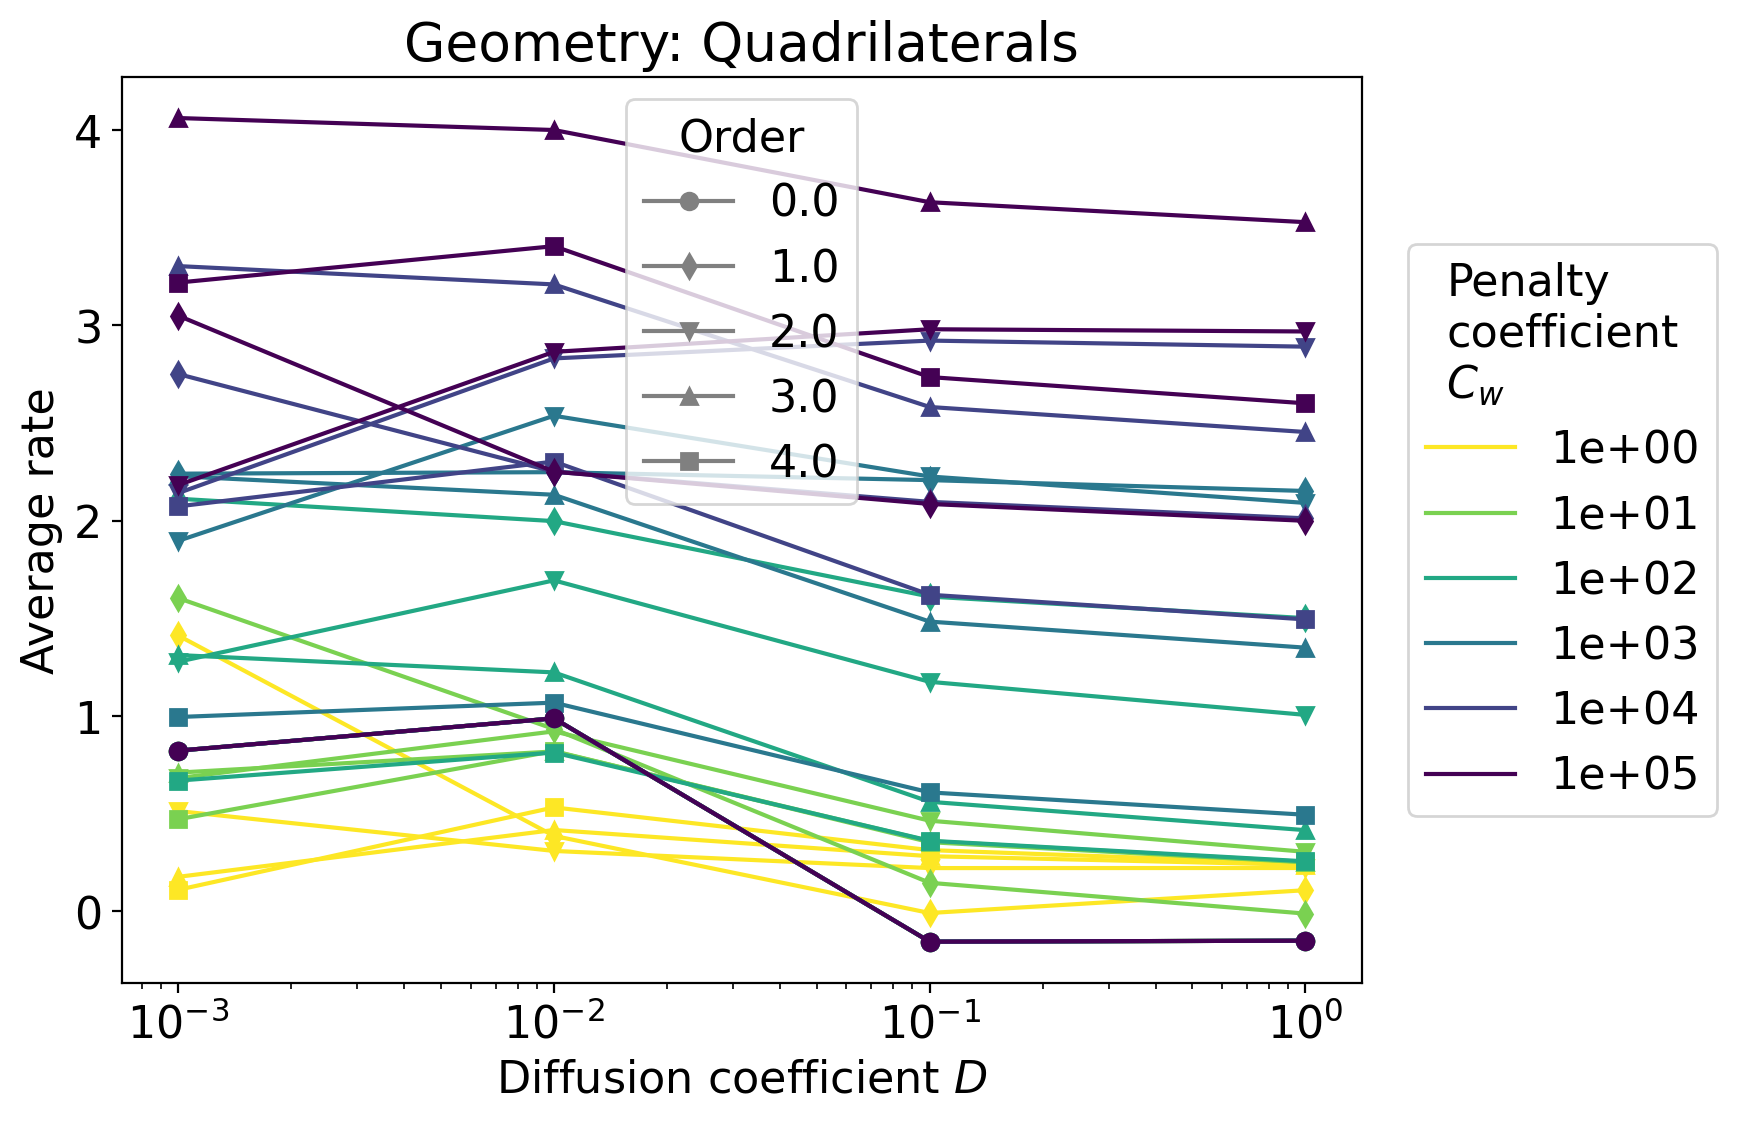
\includegraphics[width=0.4\textwidth]{../figs/parametric/advdiff_2D/ord_quarteroni1_2_4}
		&
		\vspace{0pt} 
		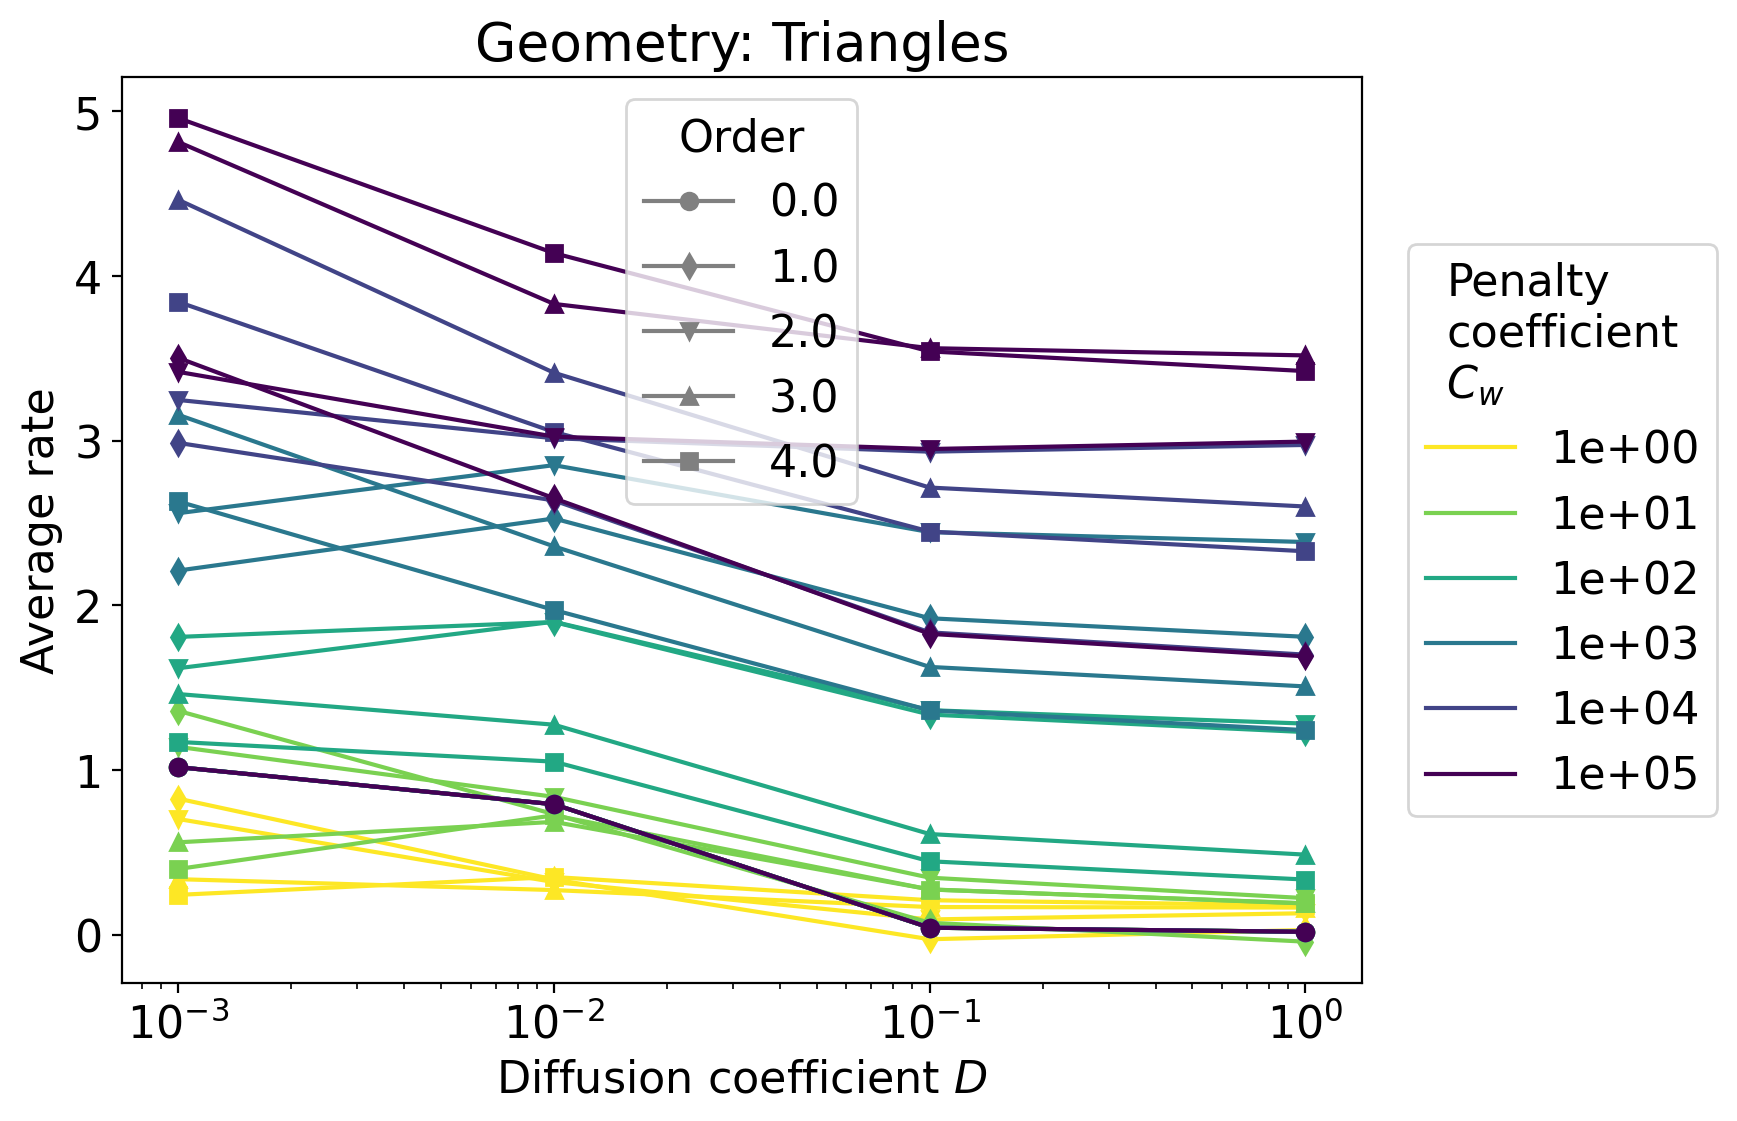
\includegraphics[width=0.4\textwidth]{../figs/parametric/advdiff_2D/ord_quarteroni1_2_3}
	\end{tabular}
	\caption{\Cref{ex:quart1}. Average convergence rates for different choice of $C_w$ 
	for quadrilaterals (left) and triangles (right).}
	\label{fig:orders_quarteroni1}
\end{figure}


\begin{figure}[h!]
	\centering
	\begin{subfigure}{.5\textwidth}	
		\centering	
		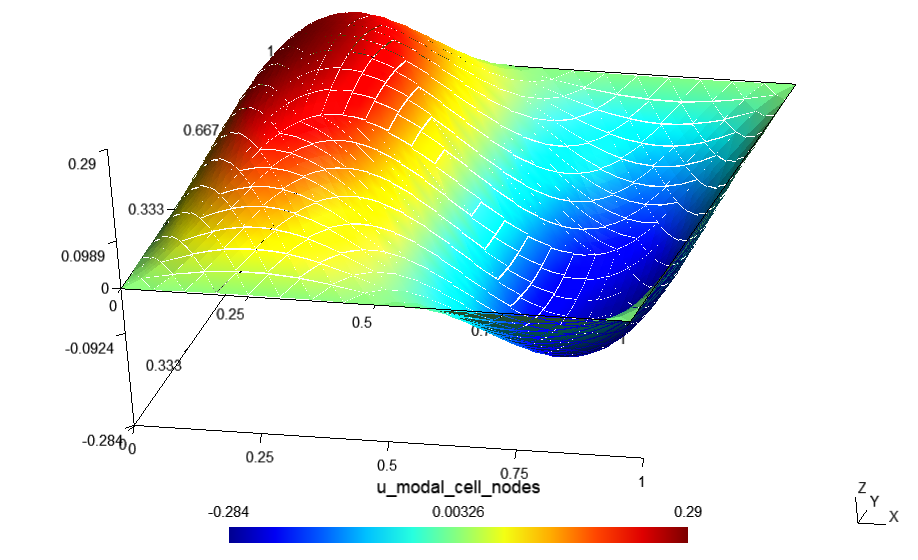
\includegraphics[width=\linewidth]{../figs/sols/quart1-03100-sol-h1024o04.png}
		\caption{$C_w = 1$}
	\end{subfigure}%
	\begin{subfigure}{.5\textwidth}
		\centering	
		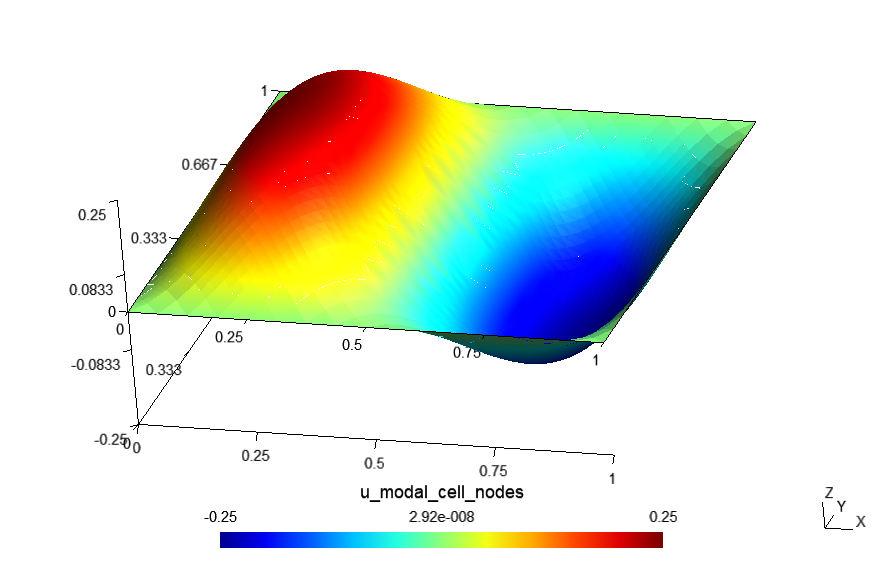
\includegraphics[width=\linewidth]{../figs/sols/quart1-53100-sol-h1024o04.png}
		\caption{$C_w = 10^5$}
	\end{subfigure}
	\caption{\Cref{ex:quart1}. Solutions on quadrilateral mesh for $D = 1$ and for 
	different values of $C_w$.}
	\label{fig:sol_quart1}
\end{figure}

\end{example}
\begin{figure}[p!]
	\centering
	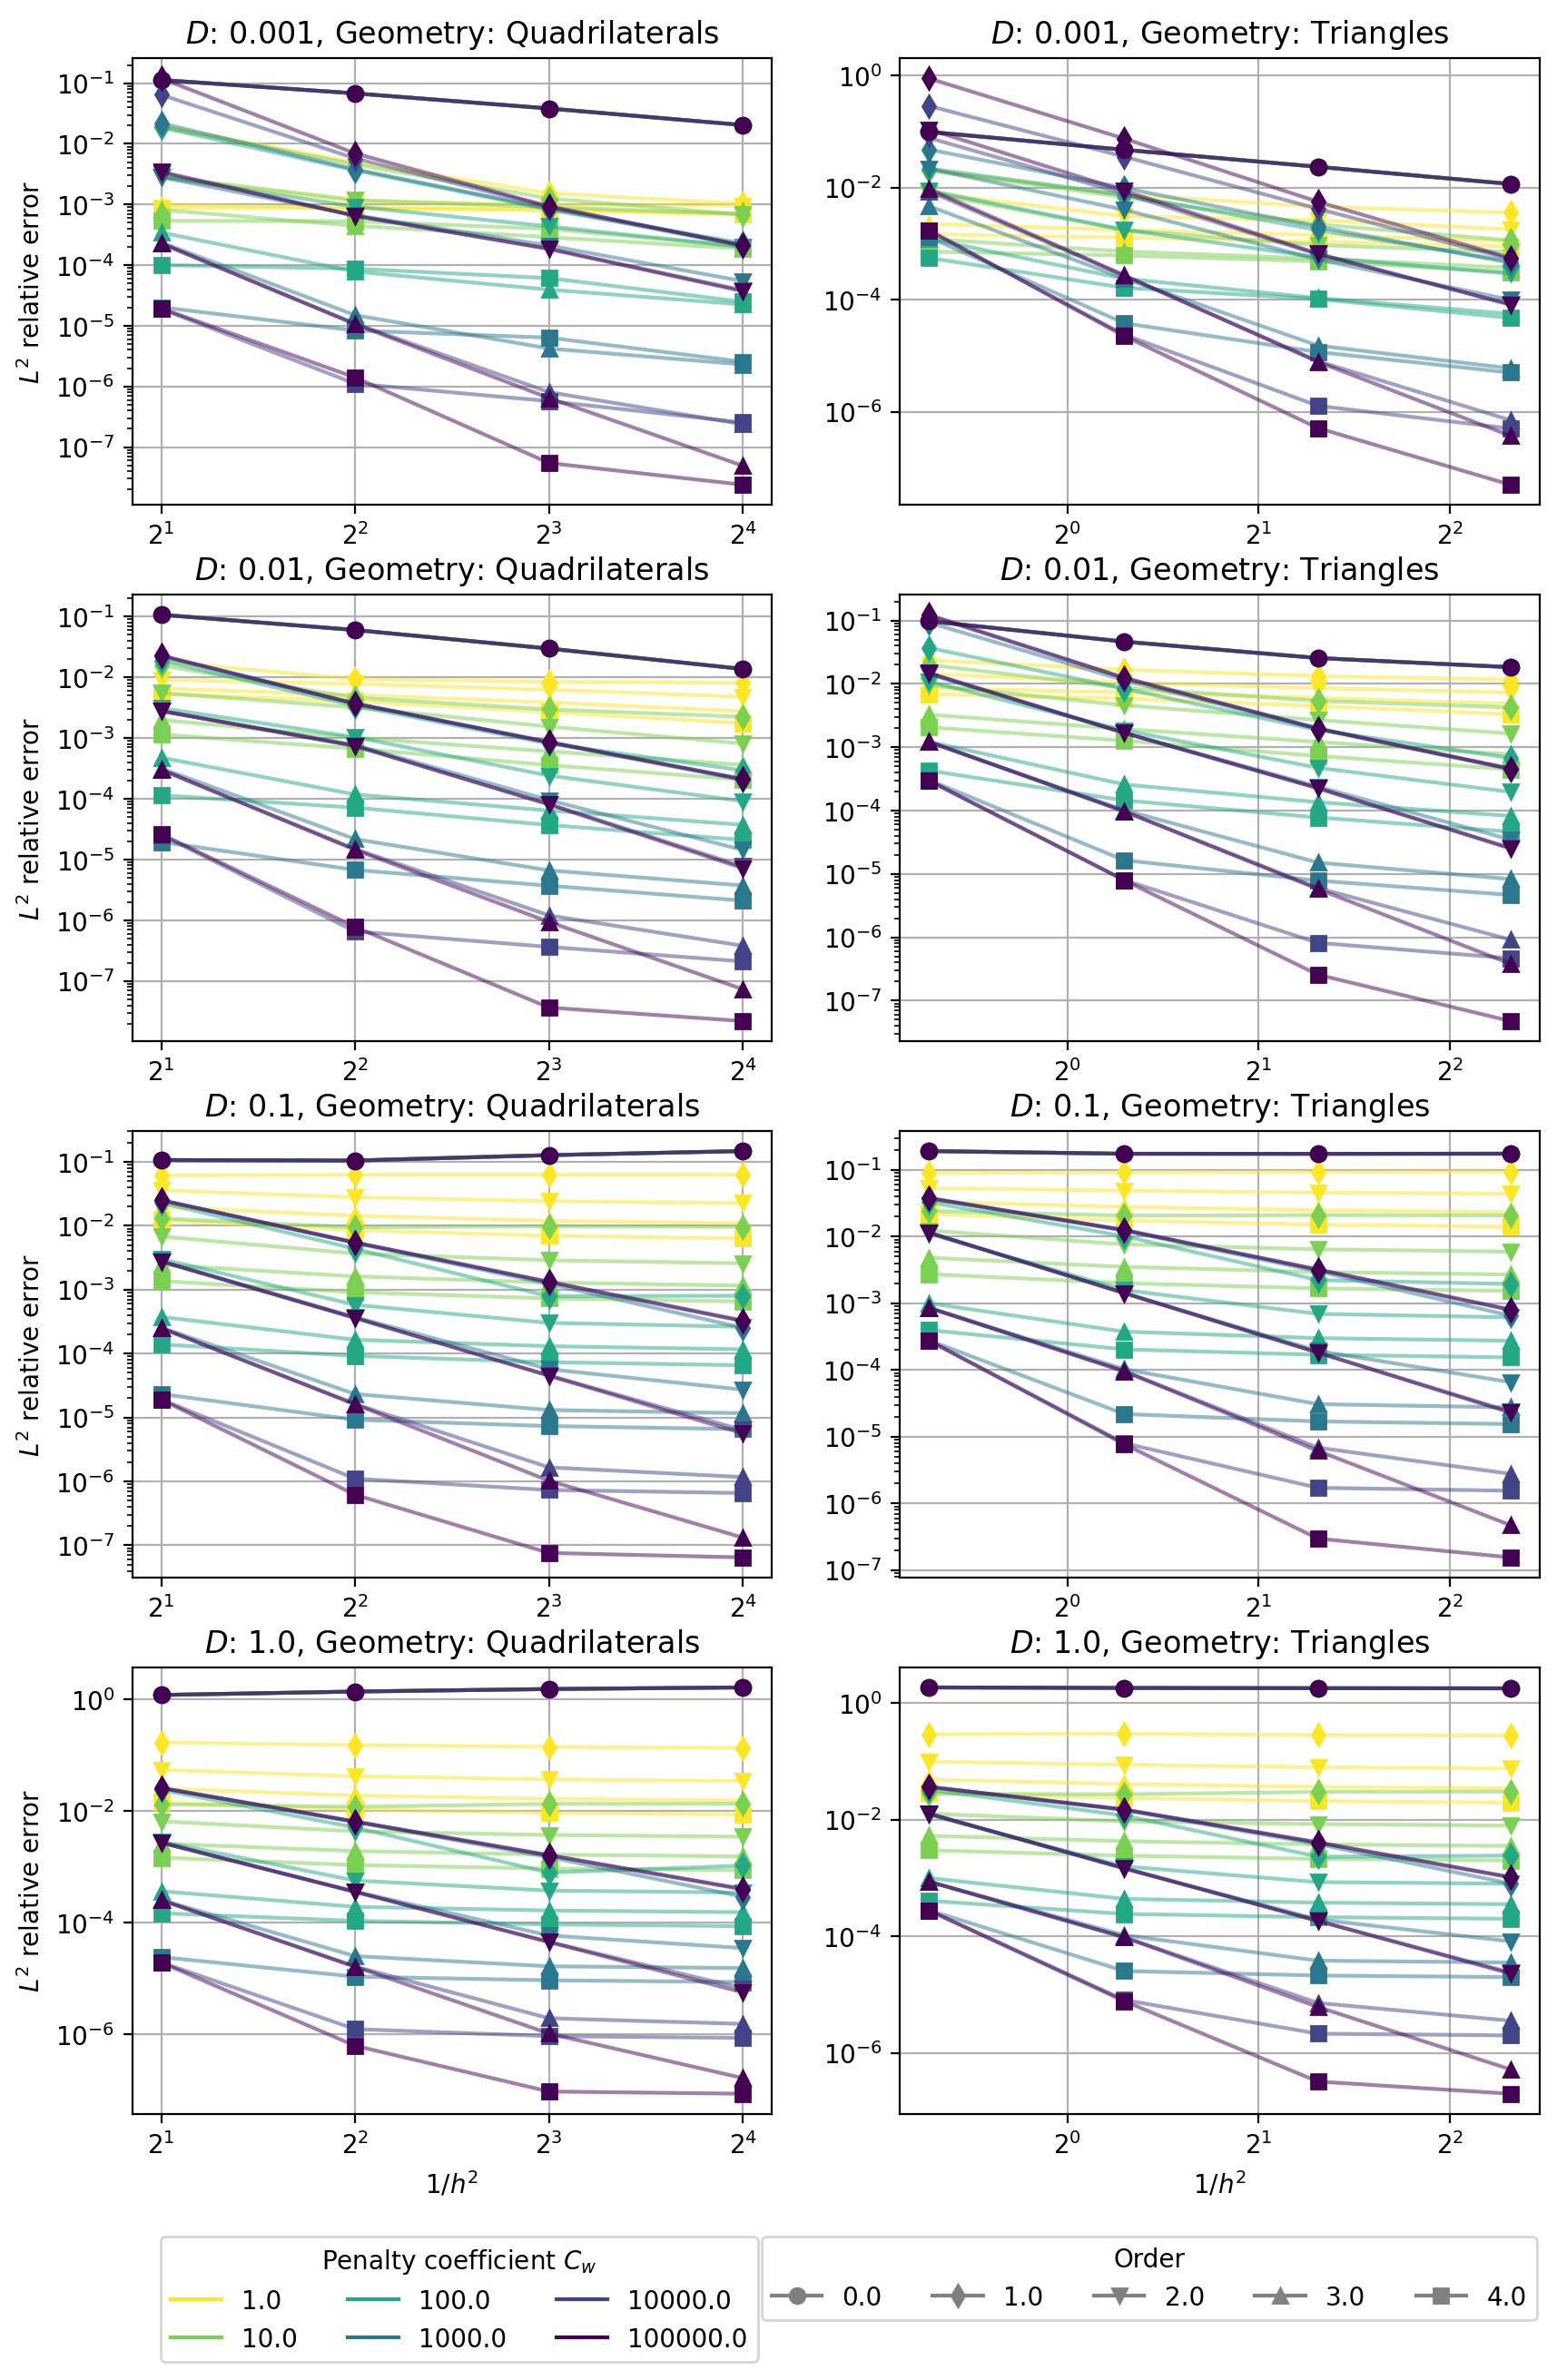
\includegraphics[height=\textheight]{../figs/parametric/advdiff_2D/quarteroni1.png}
	\caption{\Cref{ex:quart1}. Relative errors for different choices of $C_w$ for 
	quadrilaterals (left) and triangles (right).}
	\label{fig:qconv1}
\end{figure}
